\subsection{Test vehicle description}

% Why making a testchip
It is difficult to realize good measurements on an integrated circuit.
The chip is enclosed in a package, and without physical access it is impossible to measure electrical properties.
Even with physical access, placing micro-probes to contact metal connections can disturb sensitive parts of the device.
To overcome these issues, it is interesting to develop custom structures that perform the measurements directly on the chip and output the data using standard \gls{io}.
For that matter, a custom test vehicle has been designed and manufactured.

% What is in the testchip
The testchip reuses most blocks from the Everest product described previously in \ref{sec:study-real-product}.
%TODO: What is monitored
In addition, custom functions were integrated to allow the measurement and monitoring of internal parameters.
A communication system was setup to output measurement data using a few pins.

% Why monitoring a primary supply
The studied function is the primary supply of a complex automotive \gls{asic}.
This supply plays a critical role in the functionning of the entire product.
It is connected to the battery of the vehicle, and is the first block of the product to start.
It wakes up and powers all other functions inside the integrated circuit.

% Global architecture
The global architecture of the testchip (Fig. \ref{XX}) is comprised of a duplicated supply function.
The same supply block is instanciated twice on silicon.
One of them is the function under test, which is exposed to \gls{ESD} stresses and is monitored for failures.
The second one is responsible for powering the monitoring functions.
Both blocks are isolated from one another as much as possible.
The monitoring's supply is protected against disturbances to ensure good measurements.

\begin{figure}[h]
  \centering
  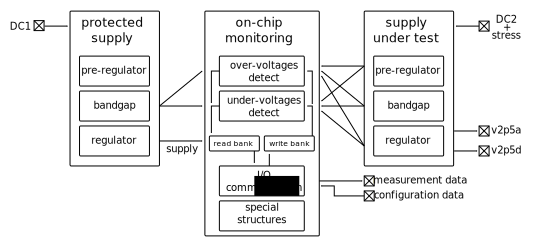
\includegraphics{src/3/figures/architecture_testchip.pdf}
  \caption{Global architecture of the test vehicle}
  \label{architecture_testchip}
\end{figure}

% What is in the monitoring system
The monitoring system is comprised of several functions.
Overvoltage and undervoltage detectors monitor voltage on nets in the supply under test.
The communication function performs a parallel to serial conversion, in order to read and write a large amount of bits using just a few pins.
Special structures for specific monitoring functions is also implemented.
Details about the monitored and monitoring functions are given in the next sub-sections.

\subsection{Monitored analog function}

The primary supply processes the battery supply in a chained fashion (see Fig. \ref{testchip_overview}).
A first block (pre-regulator) clamps the battery voltage (that can reach up to 40V) to 9V, a more acceptable voltage for the silicium technology.
This clamped voltaged is then used to power up a bandgap reference.
Once properly started, this bandgap generates a 1.23 V voltage reference, stable accross a wide range of temperature, process variation and mismatchs.
The bandgap also outputs a 10uA current reference, stable in the same conditions.

\begin{figure}[h]
  \centering
  
\includegraphics{src/4/figures/testchip_overview.pdf}
  \caption{Architecture of the studied functionnality}
  \label{testchip_overview}
\end{figure}

After the bandgap, a \gls{ldo} regulator relies on the voltage reference to generate a stable 2.5V supply voltage, able to deliver and sustain up to 20mA.
This first regulator is connected externally to a 100nF decoupling capacitor to absorb peak currents and achieve stability.
This supply is used to supply most analog (digital ?) functions inside the integrated circuit.

A second regulator performs the same task, but starts with a delay compared to the first one.
It also ouputs a 2.5V supply, that powers digital logic inside the circuit.

In case of failure, the primary supply can cause the entire product to shut down.
Indeed, this entire system requires soft-start behavior to avoid generating harmful voltage spikes to powered functions.
This functionnality enforces the system to start on a \br{long} period of time, in the order of a hundred microseconds.

When the system is stressed with an \gls{esd}, voltages and currents are fluctuating inside the block.
Under certain conditions, and especially important stress levels, the block will detects some nodes going in undervoltage or overvoltage.
This will cause the block to go into safe or protected mode, where it will restart because the functionnality cannot be assured properly.
The direct consequence is that the block will require again a hundred microseconds to be again in normal operation mode.

This failure can in a first time be observed in simulation.
An \gls{ESD} is superimposed on the DC battery voltage.
This is the most likely entry point for a stress, because the \gls{IC} exposes a pin to the external workd and is usally connected to the battery via a long cable
To detect is a block reset happened, the voltage on the first voltage regulator is observed.
Fig. X shows the stress waveform on the input.

STRESS WAVEFORM INPUT

Fig. X shows a simulation where a small glitch can be observed on the regulated output, but without clear reset or soft-failure signature.
In this case, the block and the rest of the product is most likely not affected by the ESD.

WAVEFORM OUTPUT NO RESET

Fig. X shows a simulation where a clear reset hapened.
The output voltage is maintained by a 100nF capacitor.
However, it clearly goes down \br{after} the \gls{esd} and rises slowly afterward, a sign that the block went into full reset and restard.

WAVEFORM OUTPUT RESET

By going inside the \gls{IC}...

bandgap, voltage ref, current ref, etc

DISCUSSION AROUND INCREASE OF FAILURE LENGTH after each stage of the chain

\subsection{Voltage monitoring}

% What are the OV/UV detectors made of
Overvoltage and undervoltage detectors are implemented with fast latched comparators.
The reference voltages for these comparators come from the protected supply.
The comparators monitor several key voltages inside the supply under test.
The output of these latched comparators form a register bank of 35 bits.

%TODO: Detail

\subsection{Communication system}

% What does the comm IO
The monitoring system also provides a bidirectionnal communication system.
It is designed to read with a single pin the values from the comparator register bank.
It also supports writing to a second register bank, that is used in the monitoring system for configuration.

%TODO: Detail

\subsection{On-chip near-field current sensors}

To be done
%TODO: Refer to PhD Alain
%TODO: Use document These/07
